\section{Monitoring du bus mémoire}\label{sec:yamb}


Cette section présente l'outil YAMB (\textit{Yet Another Memory Bandwidth profiling tool}). YAMB établit le profil de chaque contrôleur de mémoire en mesurant le nombre de transactions (lecture et écriture) ainsi que le nombre d'évènements \textit{miss} dans le dernier niveau de cache (LLC). Ensuite, il utilise un script python pour dessiner un graphique montrant l'évolution des trois métriques.

\begin{figure}[h!]
\center
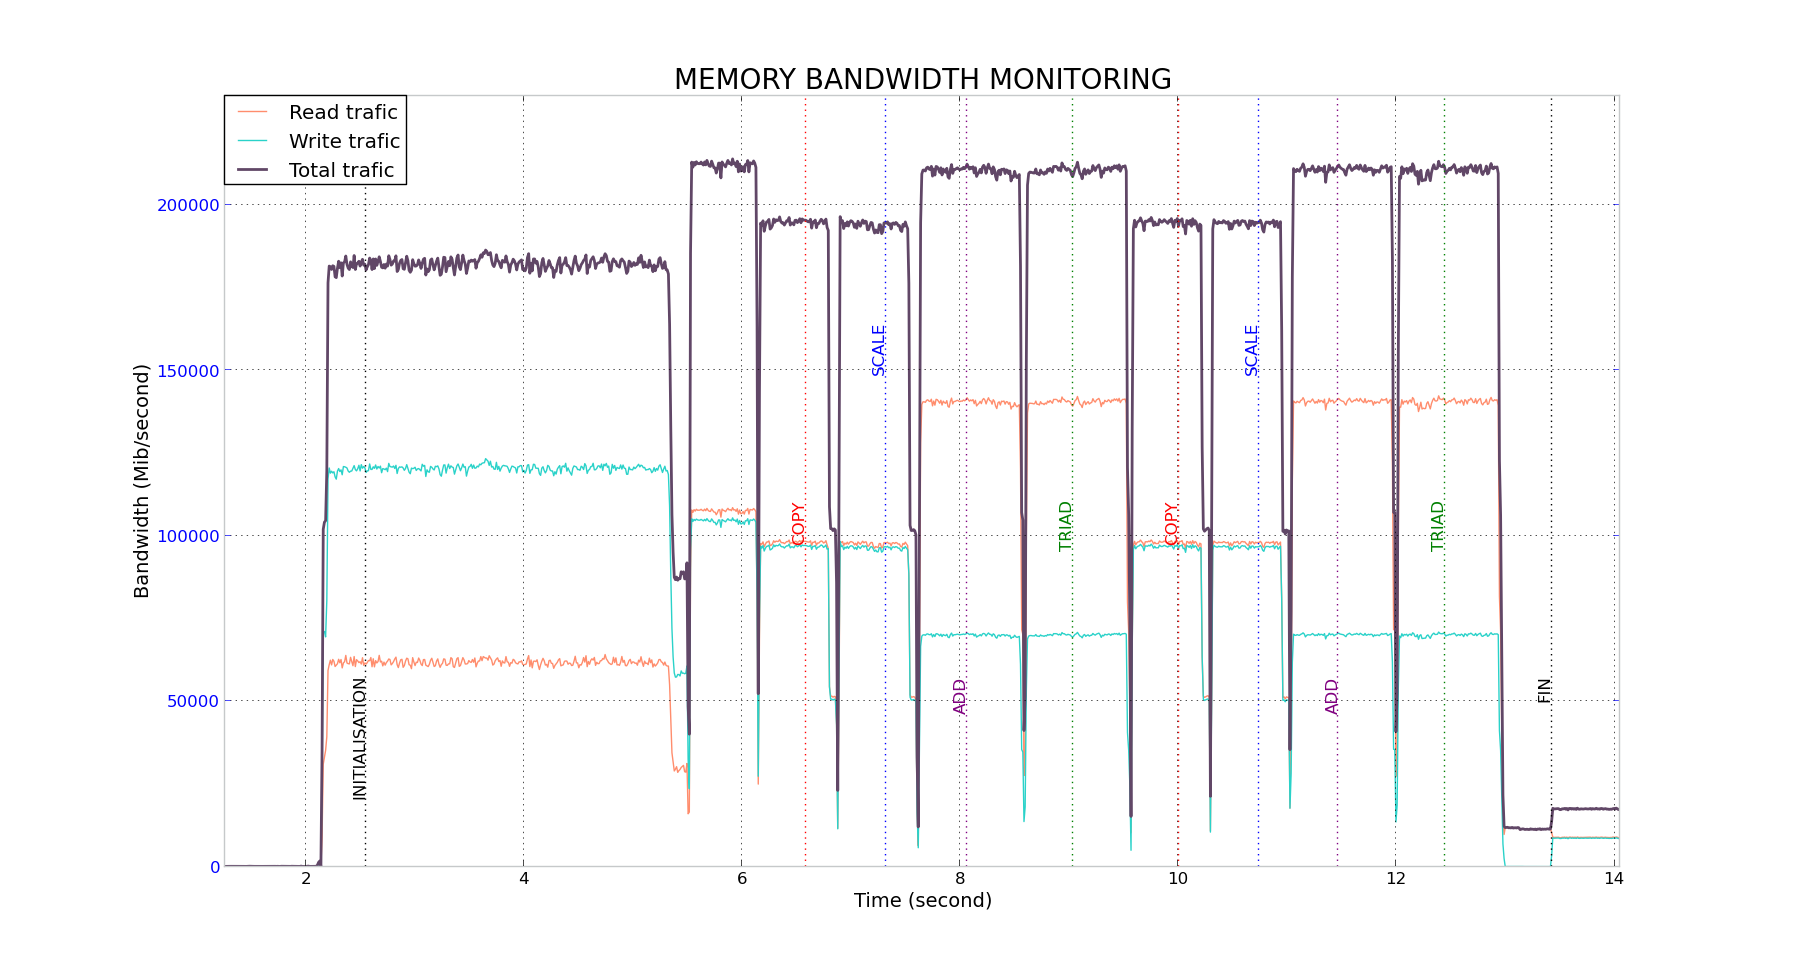
\includegraphics[width=16cm]{images/yamb_stream.png}
\caption{\label{pic:yamb_stream} Exemples d'utilisation de l'outil \texttt{YAMB} pour suivre l'activité du bus mémoire lors de l'exécution du benchmark \texttt{STREAM} pour deux itérations des 4 noyaux de calculs: \texttt{copy}, \texttt{scale}, \texttt{add} et \texttt{triadd}.}
\end{figure}




\subsection{Introduction}
%%%%%%%%%%%%%%%%%%%%%%%%%%%%%%%%%%

    \subsubsection{Motivation}
     %%%%%%%%%%%
     
        Comme présenté dans le \autoref{chap:sota:materiel}, le bus mémoire d'une architecture Von Neuman est le principal goulot d'étranglement des performances des applications de calculs intensifs\cite{Drepper2007}. Le bus mémoire est une ressource partagée par les coeurs d'un même processeur. La mauvaise utilisation de celui-ci par un coeur affecte la performance des autres. Nous observons une augmentation du nombre de coeurs sur les processeurs de dernière génération sans réelle évolution de la performance du bus mémoire. Cette disparité résulte en une augmentation d'accès concurrents à cette ressource partagée limitant la performance des applications. Il est donc primordial de s'assurer de son utilisation optimale (saturation et transferts de données utiles). Pour s'en assurer, il n'est pas possible de réaliser une mesure sur la totalité de l'application (ou d'un noyau de calculs). En effet, une application peut être limitée par la performance du bus, sans qu'il soit saturé. En effet, le déclenchement des accès mémoire par le processeur n’est pas toujours optimal pour saturer le bus mémoire sur la totalité de l'exécution. Par exemple si les accès sont tous réalisés au même moment, le bus peut être saturé pendant un court instant et être ensuite inutilisé. Sur la totalité de l'exécution, on obtiendra une mesure qui indiquera que le bus n'est pas saturé alors qu'il s'agit bien du goulot d'étranglement des performances de l'application. Le bus mémoire étant une ressource critique, il doit être utilisé pour transférer le plus possible de données utiles. Les transferts entre la mémoire et le processeur se font  par paquet (ligne de cache). Il est primordial que le maximum des données présent dans cette ligne de cache soit utilisées pour un calcul lorsque celle-ci est transférée vers le processeur. Pour cela, une adaptation des structures de données peut être nécessaire.
    
    \subsubsection{Objectifs}
    %%%%%%%%%%%
    
        L'objectif de l'outil présenté dans cette section est de répondre aux deux prérogatives indiquées dans précédemment: saturation du bus et utilisation effective. Pour y répondre, l'utilisateur doit posséder un outil lui permettant de suivre son activité avec une résolution fine (de l'ordre de la milliseconde). L'outil en question doit pouvoir distinguer les accès réalisés en lecture et en écriture pour pouvoir s'assurer de l'utilisation effective du bus. Cette méthodologie est présentée dans la section \autoref{sec:smm}.
        
        
        \paragraph{Travaux existants.} Le développent d'un tel outil a déjà été envisagé dans la littérature, mais aucun ne correspond aux critères fixés dans le début de ce chapitre (codes libres de droits, portables, ne nécessitant pas de privilèges administrateur (\textit{root})). 
        Intel propose deux outils, Intel VTune et Intel MBM. Le premier est un outil propriétaire nécessitant une licence payante. Le deuxième est proposé en libre accès sur le dépôt en ligne d'Intel\footnote{Intel MBM - \url{https://github.com/intel/intel-cmt-cat/wiki}} mais n'est compatible qu'avec des architectures Intel. 
        L'outil \textit{Likwid} propose de mesurer les données transférées (GB) et leur débit (GB/s) pour un noyau de calcul. Il peut aussi générer des traces pour suivre plus précisément l'utilisation du bus mémoire, mais l'outil de visualisation des données n'est plus supporté.
        D'autres travaux tels que \textit{Memguard}\cite{Yun2013} mesurent le nombre de \textit{miss} dans le dernier niveau de cache pour en déduire le trafic du bus mémoire. Malheureusement, avec la complexification des architectures et l'utilisation constante des unités de préchargement mémoire, certains transferts mémoires sont réalisés avant qu'un évènement \textit{miss} ne soit déclenché. Il n'est donc plus possible de mesurer le trafic mémoire avec ces techniques-là. 

    \subsubsection{Verrous}
    %%%%%%%%%%%
        
        
        Le système d'exploitation n'a généralement pas connaissance de l'évolution des accès mémoire, contrairement à d'autres ressources comme les I/O où le système d'exploitation réalise l'intermédiaire avec l'application. Mis à part certaines tâches comme la gestion des pages, les accès mémoire sont réalisés par le contrôleur mémoire. Comme étudié dans la \autoref{sec:edl_perf_uncore}, ces compteurs sont situés sur les PMU \textit{uncore}. Sur des architectures modernes telles que les processeurs Intel Skylake, ces compteurs comptent précisément tous les accès mémoire réalisés en distinguant la lecture et  l'écriture. Cependant, comme les compteurs ne sont associés à aucun coeur, il est impossible de faire correspondre un accès mémoire au coeur et donc au processus qui en est responsable. Notre outil a pour objectif d'analyser l'activité d'applications HPC qui utilisent généralement tous les coeurs des processeurs pour la même application. Cette particularité n'est donc pas un verrou majeur pour notre développement. Pour des outils nécessitant plus de précision \cite{Larysch2016}, l'utilisation de ces compteurs n'est cependant pas possible. Les moyens disponibles pour les programmer sont complexes et propres à chaque architecture. Le développement d'un outil utilisant une programmation directe des compteurs rend très difficile la portabilité de l'outil sur différentes architectures.
        
    

\subsection{Développement}
%%%%%%%%%%%%%%%%%%%%%%%%%%%%%%%%%%

    \subsubsection{Choix de l'interface}
    
    
        \paragraph{Choix de l'interface.}  
        
            De nombreux outils et interfaces ont été développés pour accéder aux compteurs matériels avec leurs avantages et leurs inconvénients. Les principales contraintes de nos développements sont la portabilité des outils et l'accès libre aux sources. Likwid et \textit{Perf Events} sont les outils répondant au maximum des critères de développement énoncés précédemment. Cependant, l'outil de visualisation de Likwid n'est plus supporté. Pour ces raisons et afin d'éviter une surcouche supplémentaire, nous avons choisi de développer nos outils en nous basant sur le système de suivi de performance \textit{Perf Events}. En effet, son intégration dans le noyau lui assure une certaine pérennité et il permet d'utiliser des évènements natifs lorsque les noms symboliques ne sont pas supportés. Ainsi, nous nous assurons un maximum de compatibilité avec les architectures émergentes.
            
            Bien qu'il s'agisse avant tout d'un outil d'espace utilisateur, la commande perf fait partie du noyau Linux du point de vue du développement. Faire partie de Linux assure une haute exigence du développement du code ainsi qu'un support au fil des versions du noyau. Lorsque le noyau supporte le nom symbolique des évènements, \textit{perf} est très simple à utiliser. Dans le cas contraire, \textit{Perf Events} offre la possibilité aux utilisateurs expérimentés d'encoder leurs propres évènements.
            
            L'inclusion de \textit{Perf Events} au projet Linux peut aussi être un inconvénient en rendant l'outil intrinsèquement lié à la version du noyau Linux. Ceci implique que pour utiliser les nouvelles fonctionnalités de perf il faut généralement installer la version du noyau correspondante. La deuxième difficulté vient de l'appel système \textit{perf\_event\_open}. S'il permet d'éviter à l'utilisateur d'écrire manuellement les différents bits de configuration des MSR, beaucoup de travail reste à faire pour le développeur désireux de profiler ses applications. Parce que Linux supporte de nombreux processeurs différents possédant différentes versions de PMU, les développeurs de noyau ont dû laisser la charge de beaucoup de détails de microarchitecture de bas niveau dépendant du code utilisateur. En conséquence, cet appel système est très complexe à utiliser et ne peut pas être utilisé de manière portable. Les principales difficultés consistent à trouver les événements à compter ou à échantillonner, à configurer tous les paramètres à transmettre à l'appel système et à effectuer plusieurs appels système en fonction du nombre de \textit{threads} de l'application profilée et du nombre de coeurs utilisés. Ces différentes difficultés (programmation, portabilité) ont été les principales motivations du développement d'autres outils tels que PAPI, Intel Performance Counter Monitor (PCM) ou NUMAP\cite{Selva2017}.

    \subsubsection{Perf Events}
    %%%%%%%%%%%%%%%%%%%%%%%%
     
        YAMB est plus un utilitaire pour la commande \textit{perf} qu'un outil autonome. Comme présenté dans \autoref{sec:edl_profiling_perf}, \textit{perf} est l'outil de profilage de Linux, et nous espérons que sa large disponibilité le rendra facilement utilisable par le plus grand nombre de personnes.  En raison des permissions limitées que les utilisateurs ont sur les clusters l'outil doit utiliser une interface ne nécessitant pas de droits privilégiés (\textit{root}) pour y accéder. Du fait du développement de l'interface \verb=perf_event= dans le code noyau il est possible pour l'administrateur d'autoriser les utilisateurs normaux à accéder aux compteurs. Cela peut être fait en écrivant la valeur 1 dans le fichier \verb=/proc/sys/kernel/perf_event_paranoid=.
        
        La commande \verb=perf= peut être utilisée pour programmer les PMU \textit{uncore} et accéder aux compteurs des contrôleurs mémoires. L'outil YAMB utilise cette commande pour configurer les PMU pour qu'elles comptent les transactions en cours sur chaque canal mémoire, en lecture et en écriture. La commande peut aussi être utilisée pour compter le nombre d'évènements \textit{miss} dans le cache de dernier niveau (optionnel).
        
        Le coeur de l'outil de profilage YAMB est le lancement de la commande \verb=perf= en arrière-plan et le traitement des données dans un fichier de sortie. Ensuite, un script peut être utilisé pour dessiner le graphique. 
        L'outil \verb=YAMB= reçoit deux options \verb=--start= et \verb=--stop=. L'utilisation de la première option lance la commande \verb|perf| avec les arguments adéquats en arrière-plan. L'appel du script avec l'option \verb=--stop= s'occupe de retrouver le \verb|PID| du processus de \verb|perf| pour l'arrêter et de sauver les données collectées dans un fichier. Entre ces deux appels, l'utilisateur peut exécuter son application ou attendre un certain temps:
\begin{lstlisting}[language=bash]
$ ./yamb.sh --start
$ ... sleep | run application ...
$ ./yamb.sh --stop
\end{lstlisting}
        Comme le montre l'extrait de code ci-dessus, l'avantage de cet outil réside dans la flexibilité de son utilisation. Il est courant dans le travail d'analyste de vouloir suivre l'exécution d'une application pendant une période donnée. L'exécution pouvant durer plusieurs heures, il est important que notre outil ne nécessite pas d'attendre l'exécution complète de l'application pour prodiguer ses résultats. Grâce à cette approche, l'utilisateur se connecte à un serveur durant l'exécution de l'application, lance le profiler pendant une période voulue et l'arrête pour analyser les résultats. Cette méthodologie permet de laisser l'application s'exécuter. Le code de l'application pouvant être instrumenté pour annoter le graphique de résultat, il est possible de tracer et d'identifier les parties du programme mesurée par l'outil.n.
        

    \subsubsection{Annotation}
    %%%%%%%%%%%%%%%%%%%%%%%%

        Pour aider à identifier la zone de code responsable du trafic mémoire, une librairie a été développée. Elle permet d'annoter le code d'une application (\verb=c= et \verb=fortran=) à l'aide d'un \verb=label= et d'une \verb=couleur=. La librairie ne contient que la fonction \verb=yamb_annotate_set_event= permettant d'écrire ces informations en plus d'un pas de temps dans un fichier de journal:
\begin{lstlisting}[label=lst:yamb_api ,language=C]
int yamb_annotate_set_event(const char * label, const char *couleur){
...
    m_LOG_FILE << time_step << " " << label << " " << couleur << endl;
...
}
\end{lstlisting}
    


\subsection{Résultats}
%%%%%%%%%%%%%%%%%%%%%%%%%%%%%%%%%%


    \subsubsection{Application à STREAM}
    %%%%%%%%%%%%%%%%%%%%%%%%

        Cette section présente un exemple d'utilisation de \verb=YAMB= appliqué au benchmark \verb=STREAM=. Pour mieux comprendre l'évolution du trafic mémoire, la première étape est d'annoter les différentes parties du codes intéressantes. Pour cela, nous utilisons la fonction \verb=yamb_annotate_set_event= pour ajouter une trace sur le graphique lors de chaque début de benchmark. L'analyse peut ensuite être lancée avec les commandes suivantes:
    
\begin{lstlisting}[label=lst:yamb_api ,language=C]
$ ./yamb.sh --output log_stream --command ./stream.SKL.192GB
$ python ./format_log.py --data log_stream.perf.mem --annotate log_stream.annotate
\end{lstlisting}

        Le résultat de cette première expérimentation peut être vu sur la \autoref{pic:yamb_stream}. L'utilisation du graphique peut ensuite permettre d'agrandir les parties plus intéressantes comme le noyau de calcul \verb=triad=(voir \autoref{pic:yamb_stream_triad}). Grâce à la distinction entre les accès mémoire réalisés en lecture ou en écriture, nous pouvons remarquer que le ratio de transfert est de deux lectures pour une écriture.
        
        
        \begin{figure}
        \center
        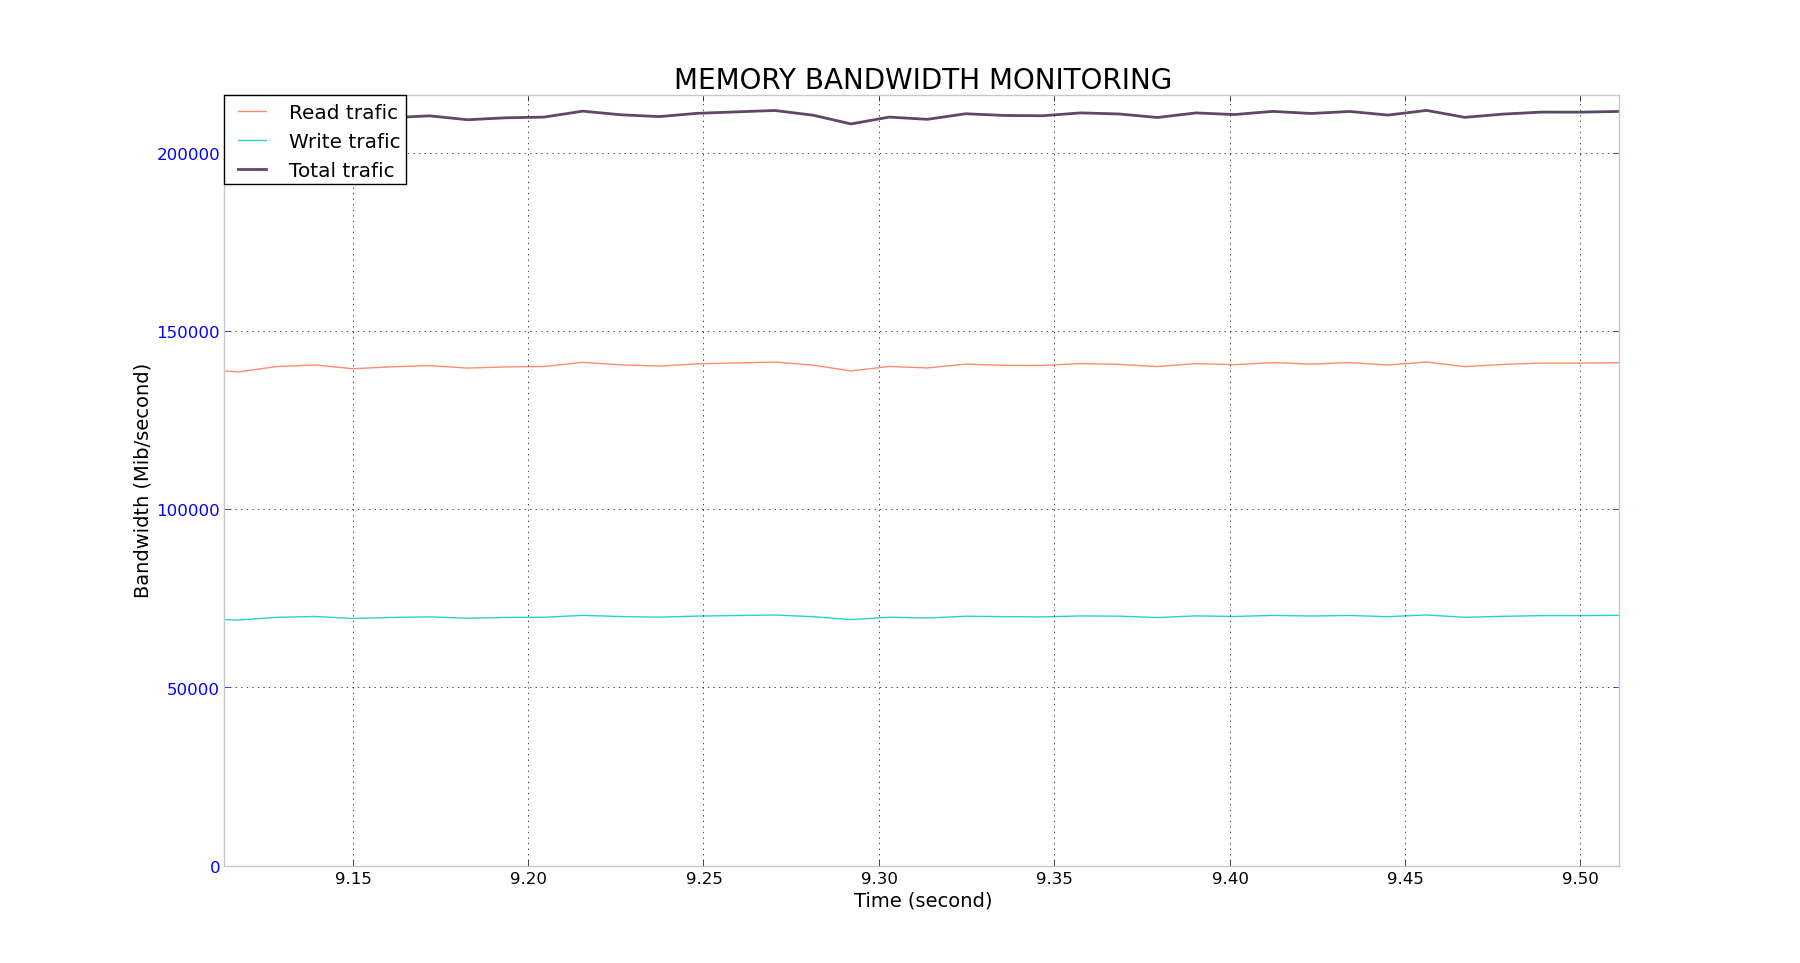
\includegraphics[width=14cm]{images/yamb_stream_triad.png}
        \caption{\label{pic:yamb_stream_triad} Profil de l'utilisation du bus mémoire lors de l'exécution de la fonction \texttt{triad} du benchmark \texttt{STREAM}.}
        \end{figure}


        \paragraph{Autres exemples.} L'outil \verb|YAMB| est utilisé à plusieurs reprises dans ce manuscrit de thèse. Une utilisation est réalisée avec le benchmark \verb=dml_mem= pour caractériser la capacité du cache de dernier niveau à stocker un jeu de données dont la taille s'approche de celle du cache (\autoref{}). Une autre utilisation est présentée dans la \autoref{chap:methodo} pour illustrer l'application de la méthodologie et de l'utilisation des ratios de lecture et écriture pour s'assurer de l'optimalité d'un code.
        
        

    \subsubsection{Mesure de l'impact sur la performance}
    %%%%%%%%%%%%%%%%%%%%%%%%
        Un défaut majeur des outils de mesure de performance est leur impact sur la performance de l'application étudiée. Nous avons réalisé plusieurs tests avec différentes fréquences d'échantillonnage pour estimer l'impact de \verb|YAMB| sur l'application mesurée. Même lorsque la fréquence la plus rapide de \verb=perf= est utilisée (100Hz), l'impact sur la performance est très faible (inférieur à 5\%). Pour une étude suffisamment précise de l'application, obtenir 100 mesures par seconde semble largement suffisant. Nous considérons que cette baisse de performance est suffisamment faible pour s'assurer que la performance mesurée est proche de la performance réelle.
        